\documentclass[aspectratio=169]{beamer}
\usepackage{simplebeamer}
% \usepackage{textgreek} % for greek letters outside of math mode. may be useful later

\begin{document}

%-------------------------------------------------
\section{My goal this summer}
%-------------------------------------------------

\begin{frame} \frametitle{\insertsection}
    \begin{center}
        \centering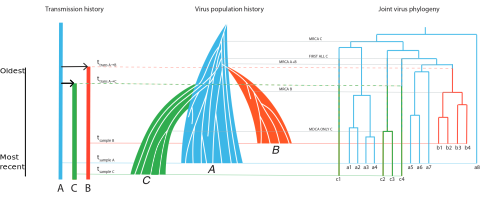
\includegraphics[width=\textwidth]{images/thomas-figure}

        Work from a phylogeny to the original transmission history

        \ftnB{Modified from Leitner et al., Curr. Opin. HIV AIDS (2019)}
    \end{center}
\end{frame}

%--------------------------------------------------
\section{Coalescent modeling}
%--------------------------------------------------

\begin{frame} \frametitle{\insertsection}

        \centering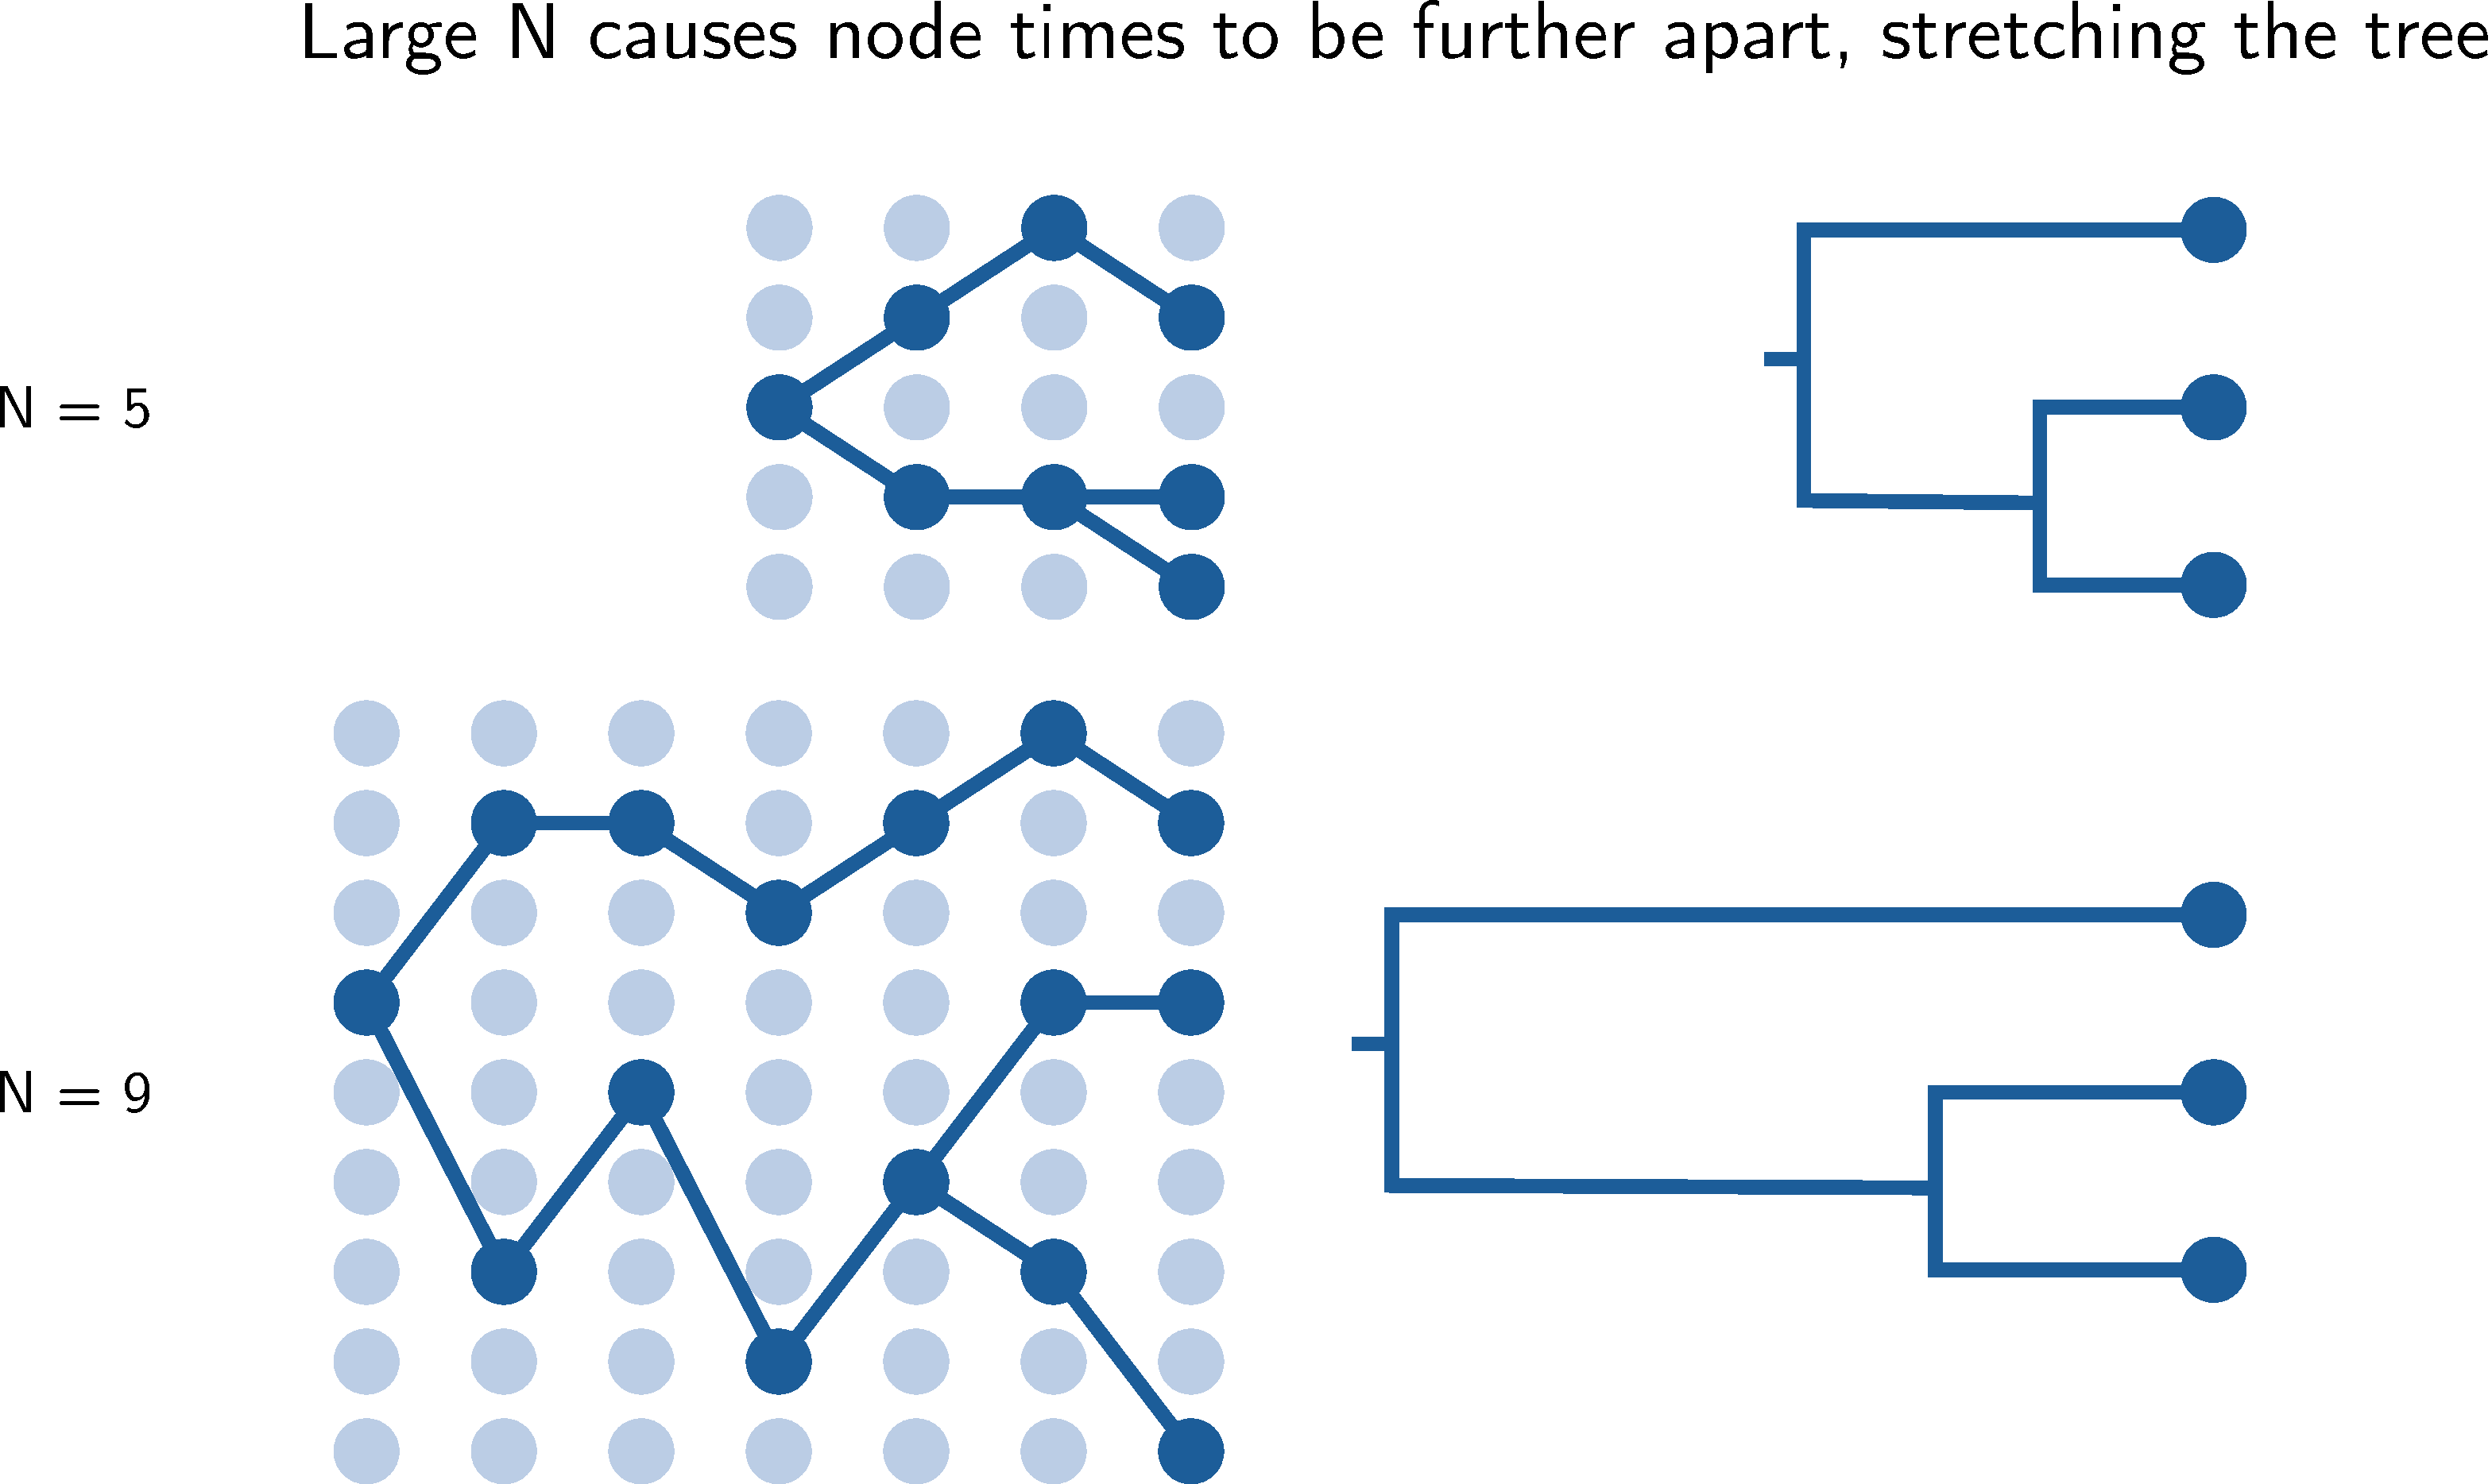
\includegraphics[width=0.8\textwidth]{images/coalescence}

\end{frame}

%--------------------------------------------------
\section{Time until first coalescence with arbitrary B}
%--------------------------------------------------

\begin{frame} \frametitle{\insertsection}

    \vspace{0.18cm}

    \centering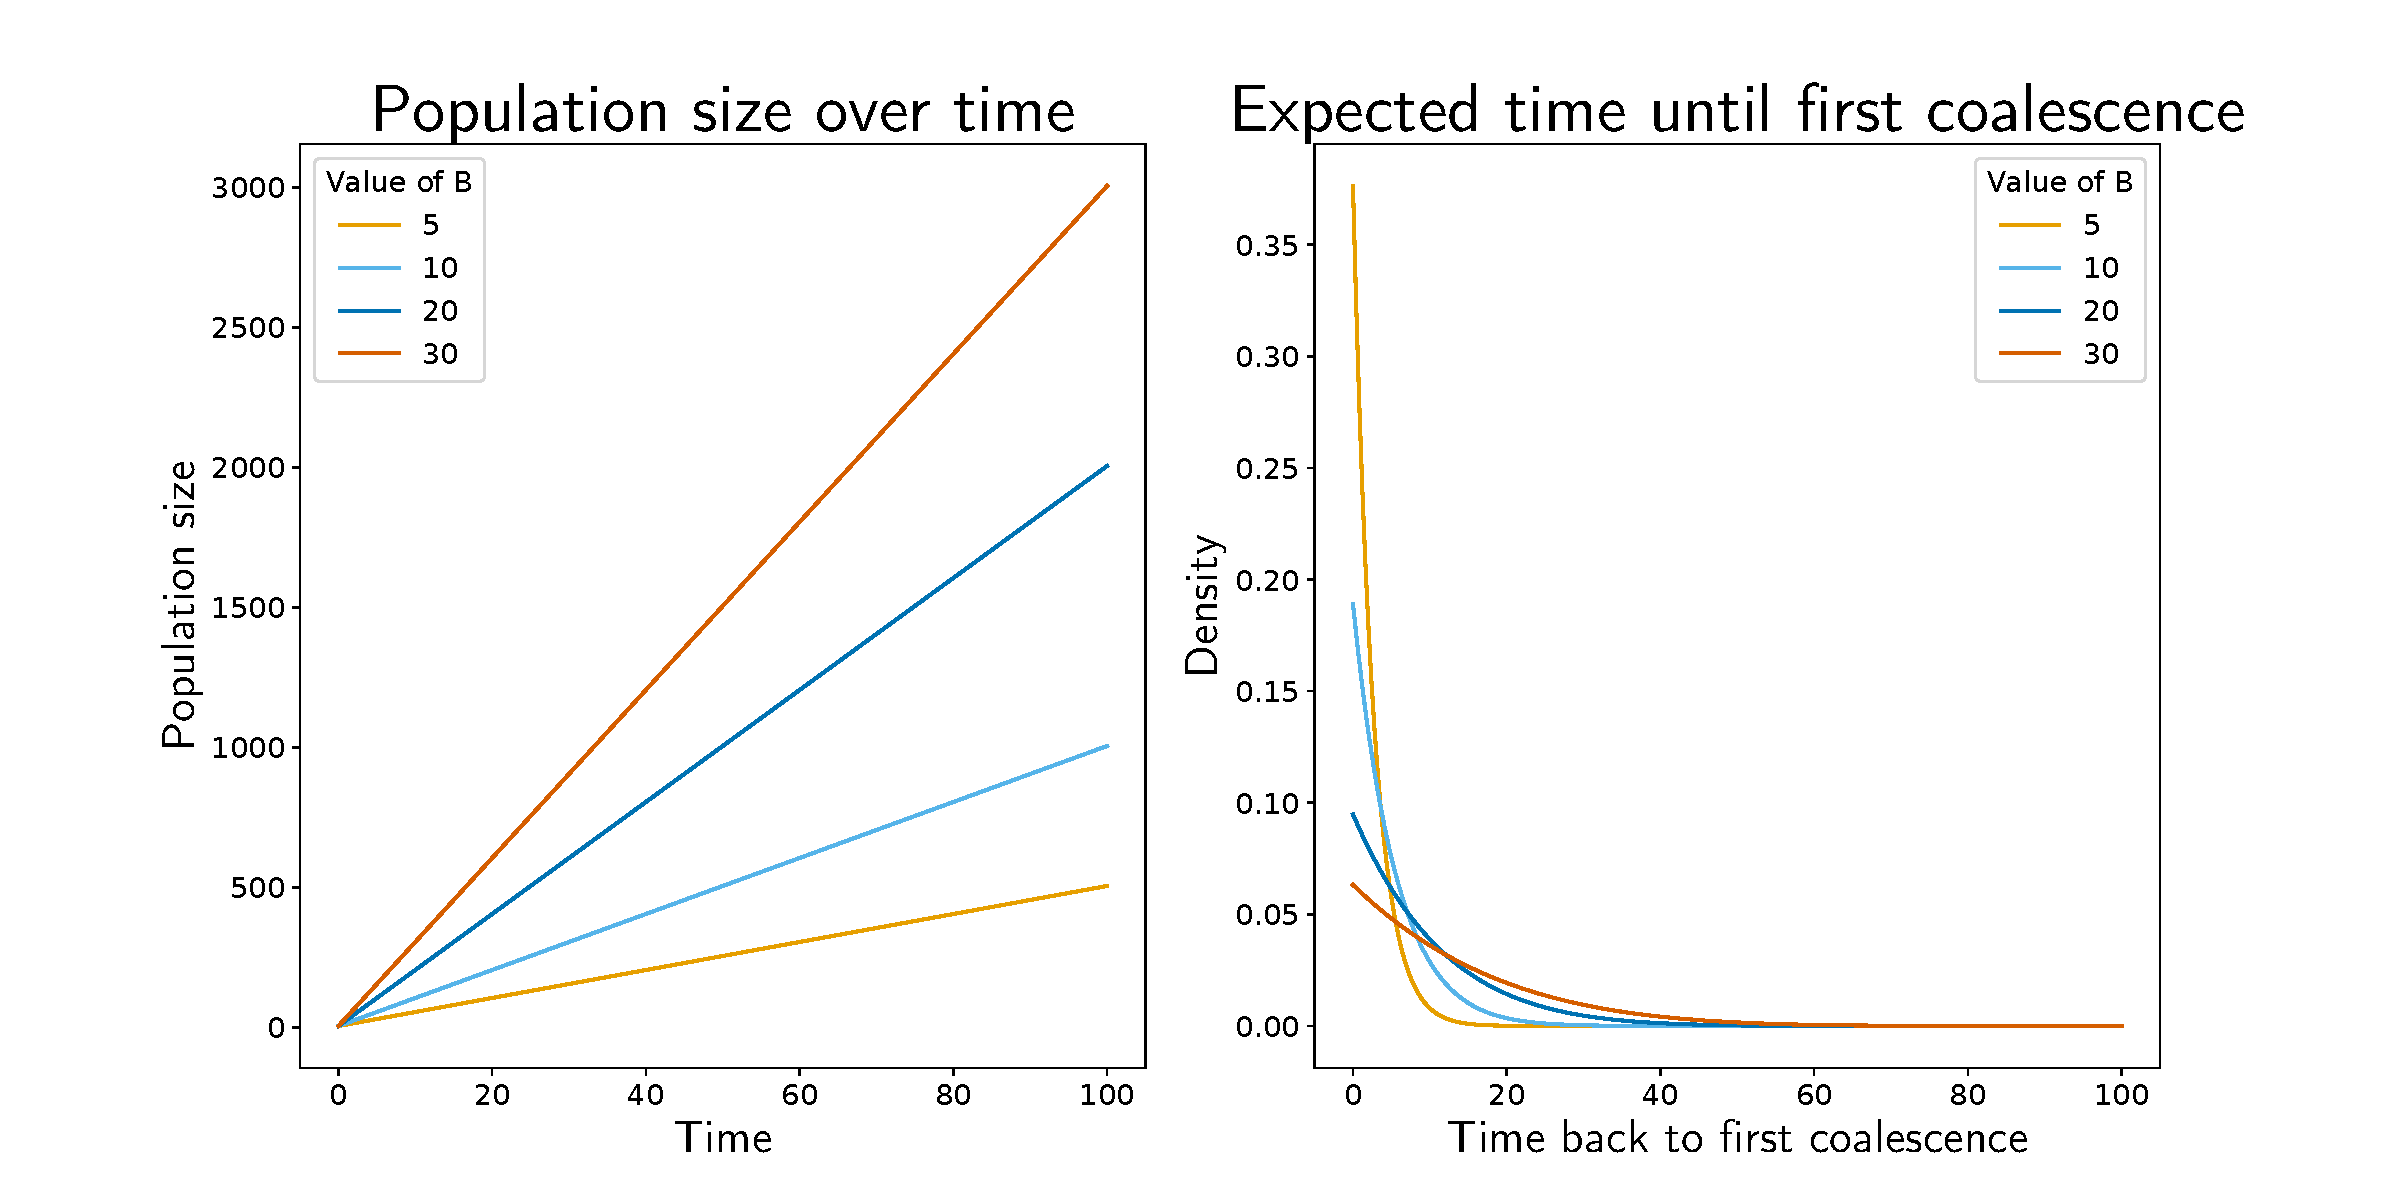
\includegraphics[width=\textwidth]{images/several-b}
        
    \ftnB{Romero-Severson et al., Mol. Biol. Evol. (2014); Shankarappa et al., Jrnl. Virology (1999); Zanini et al., eLife (2015)}

\end{frame}

%--------------------------------------------------
\section{Expected signal for transmission time with two hosts}
%--------------------------------------------------

\begin{frame} \frametitle{\insertsection}

    \centering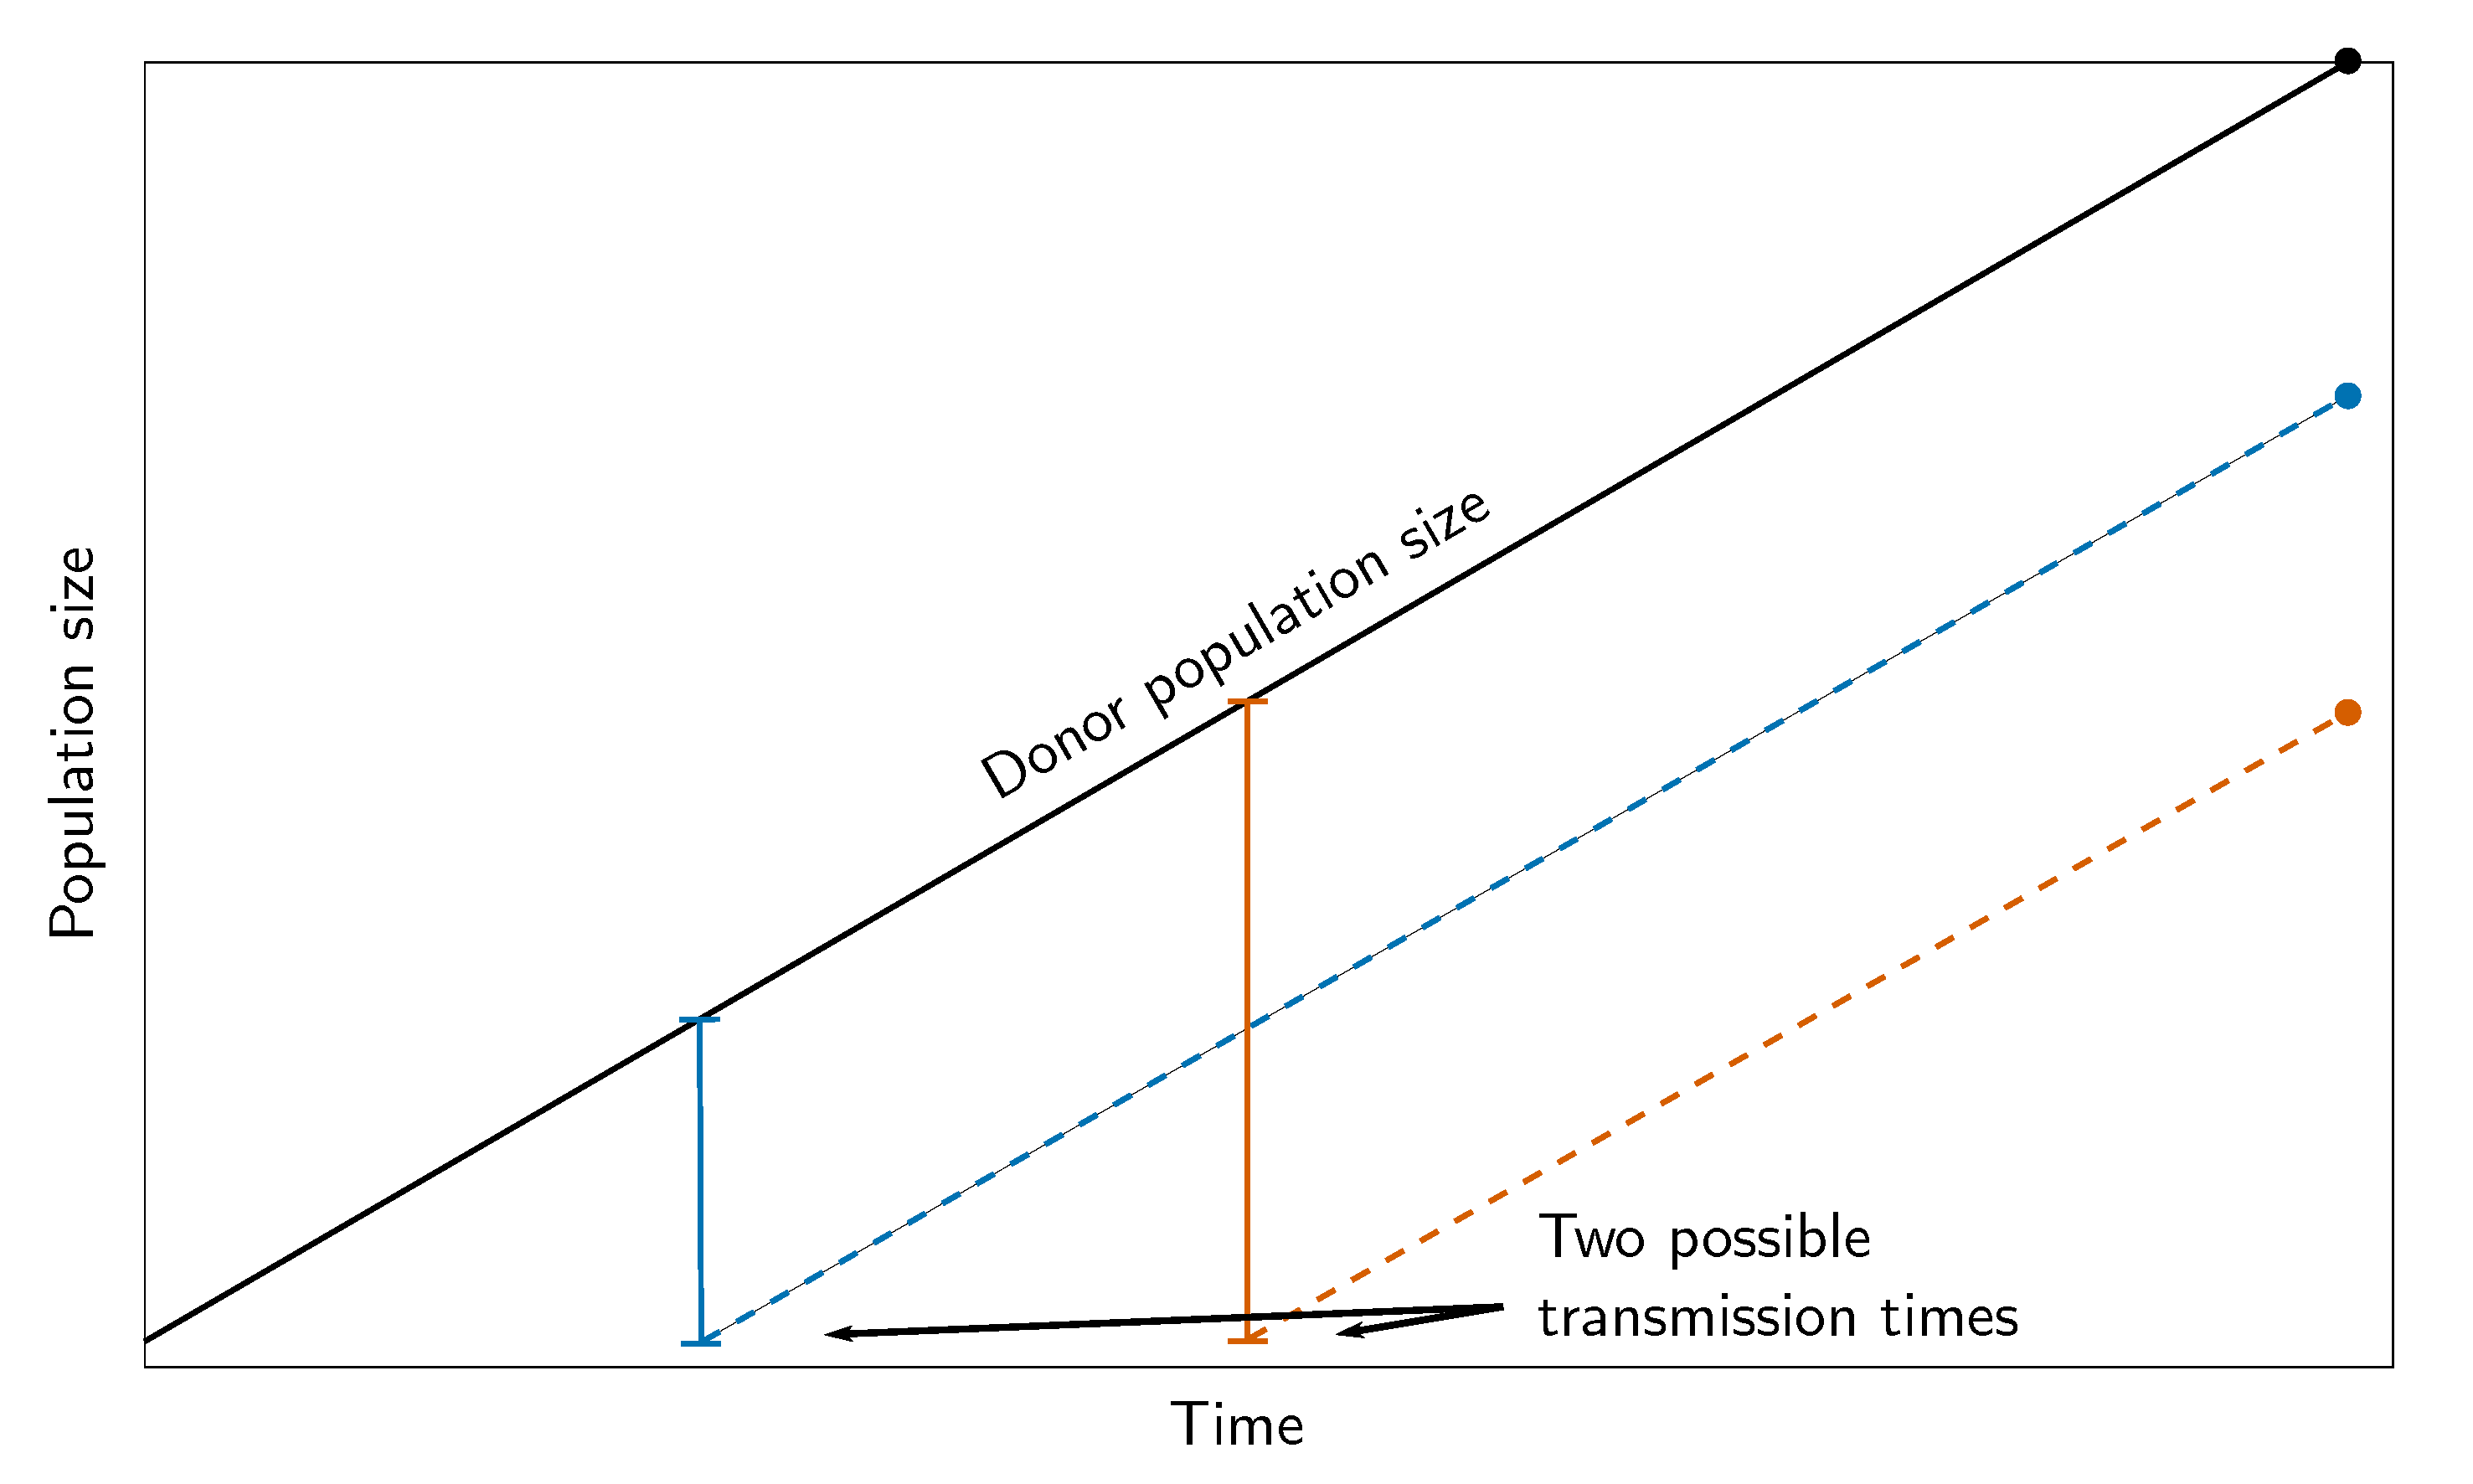
\includegraphics[width=0.8\textwidth]{images/linear-time-location}

\end{frame}

%--------------------------------------------------
\section{My results so far: Constant population size, single host}
%--------------------------------------------------

\begin{frame} \frametitle{\insertsection}

    \centering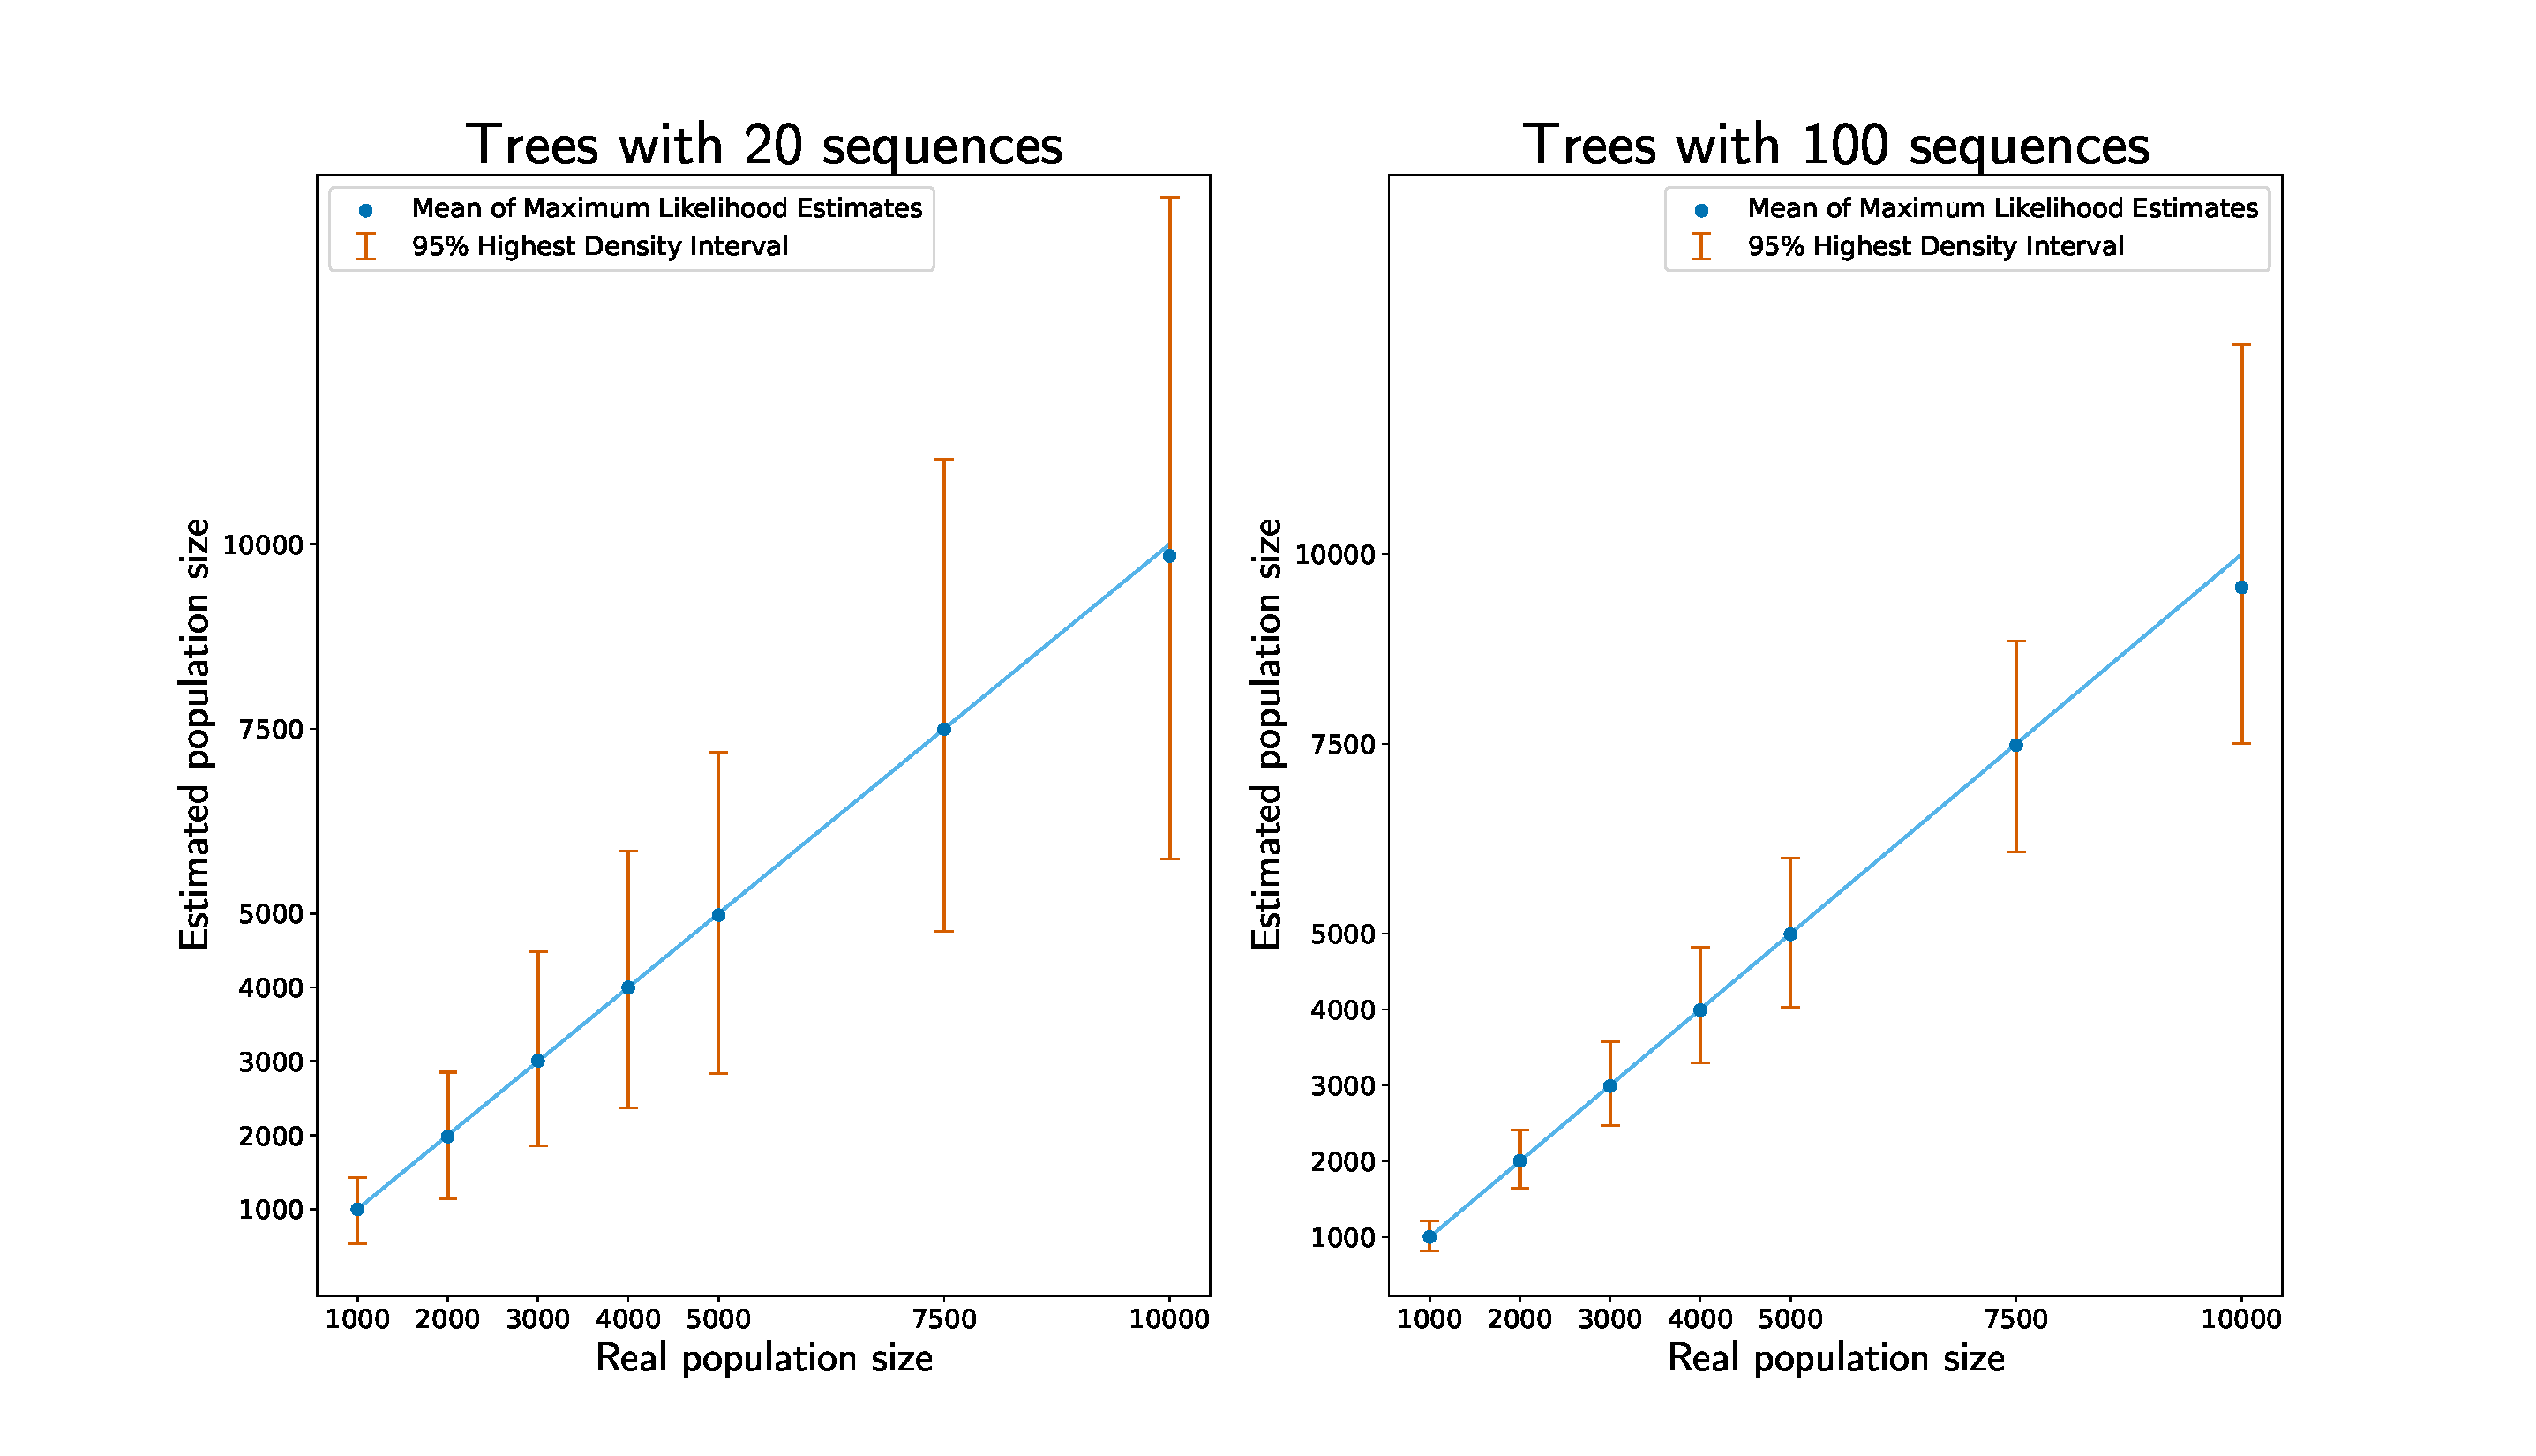
\includegraphics[width=\textwidth]{images/constant-accuracy}

\end{frame}

%---------------------------------------------------
\section{My current progress on linear populations}
%---------------------------------------------------

\begin{frame} \frametitle{\insertsection}

    \centering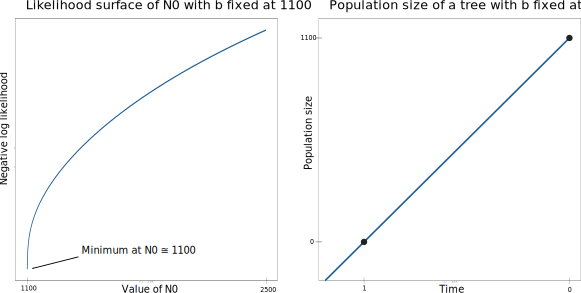
\includegraphics[width=\textwidth]{images/linear-progress}

\end{frame}

%--------------------------------------------------
\section{Attempting a grid search revealed scaling mistakes with B}
%--------------------------------------------------

\begin{frame} \frametitle{\insertsection}

    I have the high ground, bananakin!

    I can't add this image now because I can't properly git pull,
    so it will need to be last minute tomorrow morning.
    
\end{frame}

%--------------------------------------------------
\section{Next steps: Moving towards two hosts and linear population}
%--------------------------------------------------

\begin{frame} \frametitle{\insertsection}
    
    \begin{columns}

        \begin{column}{0.5\textwidth}

            \begin{itemize}
                \item{Look into incorrect population growth scaling across the project}
                \item{Instead of a grid search, explore more serious optimization methods}
                \item{Expand to a two-host problem so I can examine transmission time}
                \begin{itemize}
                    \item{Split tree by host}
                    \item{Isolate hosts until a transmission occurs}
                \end{itemize}
            \end{itemize}
            
        \end{column}

        \begin{column}{0.5\textwidth}

            \centering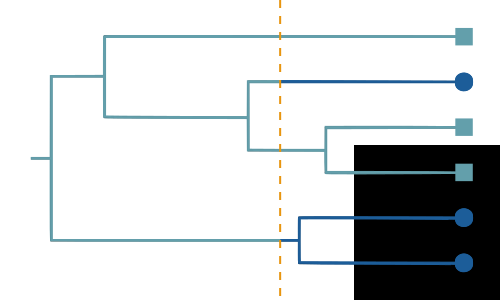
\includegraphics[width=\textwidth]{images/tree-option1}

        \end{column}

    \end{columns}
    
\end{frame}

\end{document}
